\documentclass[a4paper]{article}
\usepackage{amsmath}
\usepackage{amsthm}
\usepackage[swedish]{babel}
\usepackage[utf8]{inputenc}
\usepackage{graphicx}
%\usepackage{cite}
\usepackage[round, sort, numbers]{natbib}

\setcitestyle{square}
\begin{document}
\title{temp}
\author{Niil Ohlin}
\date{}
\maketitle

\section{The Koch Snowflake}
The \emph{Koch snowflake} one of the first fractals, is based on work by the
Swedish mathematician Helge von Koch \cite{aoeu}. It is what we get if we
start with an 
\begin{center}
	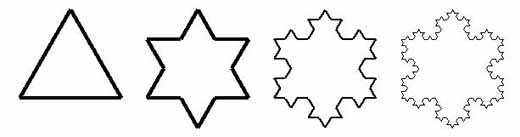
\includegraphics[scale=0.4]{snowflake.jpg}
\end{center}
Figure 1:$\quad$The initial equilateral triangle and the refinement of the Koch
snowflake after one, two, and ther iterations.\\
\\
equilateral triangle and repeat the following an infinite number of times:

\begin{quote}
\emph{Divide all line segments into three segments of equal length. Then draw,
	for each middle line segment an equilateral triangle that has the middle
	segment as its base and points outward. Finally, remove all middle segments.
	}
\end{quote}
Figure 1 shows the firstiterations in the construction. \hfill (Original)
\subsection{Two properties}
\paragraph{Theorem 1.} \emph{The Koch snowflake has infinite length.}
\emph{Proof.} Let $\Delta$ denote a triangle, with side length $s$, on which
we base the construction of a snowflake. Len $N_i$ denote the number of line
segments, and $L_i$ the lenth of the segments, in iteration $i$ of the 
construction. Then
$$
	N_n = 
	\begin{cases}
		3 &\text{if } n = 0 \text{ (i.e before any iterations), and} \\
		4N_{n-1} &\text{otherwise,}
	\end{cases}
$$
which solves to
\begin{equation}
	N_n = 3 \cdot 4^n,
\end{equation}
while
\newcommand{\uberfrac}[1]{
	= \frac {L_{n - #1}} {3^#1}
}

\begin{equation}
	L_n = \frac {L_{n-1}} {3} \uberfrac{2} \uberfrac{3} = \ldots = 
		\frac{L_0} {3^n} = \frac s {3^n}
\end{equation}
The total length
$$
	N_nL_n = 3 \cdot 4^n \frac s {3^n} = 3s \frac {4^n} {3^n} = 3s \left (
		\frac 4 3
	\right )^n.
$$
Since $4 / 3 > 1$, it follows that $N_nL_n$ tends to infinity as
$n \to \infty$, i.e. the Koch snowflake has infinite length. 
\hfill \qed
\paragraph{Theorem 2.} \emph{The Koch snowflake has finite area.}\\
\emph{Proof.} In an iteration, a triangle is added on each line segment of the
previous iterations. So, in iteration $n$, the number of new triangle
$T_n = N_{n-1}$, which, by Eq. 1, can be siplified to
\begin{equation}
	T_n = \frac 3 4 \cdot 4^n.
\end{equation}
The area $a_n$ of each such triangle, with the exception of the area
$a_0 = \frac {\sqrt 3} 4 s^2$ of $\Delta$, is one ninith of the area of a 
triangle added in iteration $n - 1$, or

\begin{equation}
	a_n = \frac {a_{n-1}} {9}
		= \frac {a_{n-2}} {9^2}
		= \frac {a_{n-3}} {9^3}
		= \ldots
		= \frac {a_0} {9^n}.
\end{equation}
%may be better to ref
This means that in iteration $n$ be Eqs. 3 and 4, the area of all added
triangles
$$
	b_n = T_na_n = \left (
		\frac 3 4 \cdot 4^n
	\right )
	\left (
		\frac {a_0} {9^n}
	\right ) = \frac {3a_0} 4 \left (
	\frac 4 9
	\right )^n
$$
All in all, after iteration $n$, the tatal area \hfill (Original)
\newcommand{\ubersum}[2] {
	\sum_{k=#2}^{n#1}
}
\begin{align*}
	A_n &= a_0 + \ubersum{}{1} b_k \\
		&= a_0 \left (
				1 + \frac 3 4 \ubersum{}{1}\left(\frac 4 9 \right )^k
			\right ) \\
		&= a_0 \left (
				1 + \frac 1 3 \ubersum{-1}{0}\left(\frac 4 9 \right )^k
			\right ) \\
		&= a_0 \left (
				1 + \frac 3 5 \left ( 1 - \left( \frac 4 9 \right )^n \right )
			\right ) \\
		&= \frac {a_0} 5 \left (
				8 - 3 \left ( \frac 4 9 \right )^n
			\right )
\end{align*}
Now, since
$$
	\lim_{n \to \infty} 3 \left ( \frac 4 9 \right )^n = 0,
$$
it follows that $lim_{n \to \infty} A_n = \frac {8a_0} 5$, i.e. the Koch 
snowflake has finite area. \hfill \qed

\bibliography{derp}{}
\bibliographystyle{plain}
\begin{thebibliography}{9}
	\bibitem{aoeu}
		Helge von Koch,
		\emph{Sur une courbe continue sans tangente, obtenue par une
		construction géométrique élémentaire},
		Arkiv för matematik, astronomi, och fysik, Kngliga Vetenskapsakademien.
		1,
		681 - 702,
		1904
\end{thebibliography}


\end{document}
